\chapter{Examples}\label{example}
\section{Cuneiform tablets}\label{cuneiform}
%At the moment the applicational focus lies on cuneiform tablets so there exists the possibility to calculate and export drawings as vector graphics. Furthermore methods known from image processing are implemented as well to remove measurement errors from the 3D data. 
Here is first and detailed example what can be done with \GigaMesh to get a feeling on how to use the program. However,  some of the pictures of the illustration may be outdated due to the ongoing development of the program.
As the main focus lies on the visualization of cuneiform script this section will show how to visualize the 3D model of a cuneiform tablet and how to do a fat-cross view.

%\newcounter{stepcount}
%\setcounter{stepcount}{1}
%\renewcommand{\thestepcount}{\textbf{Step \arabic{stepcount}\qquad}}

%\paragraph*{\thestepcount \usecounter{stepcount}\addtocounter{stepcount}{1}}
\paragraph*{Step 1}
Start \GigaMesh and browse to open the 3D model to be visualized. 
\begin{figure}[H]
\begin{center}
    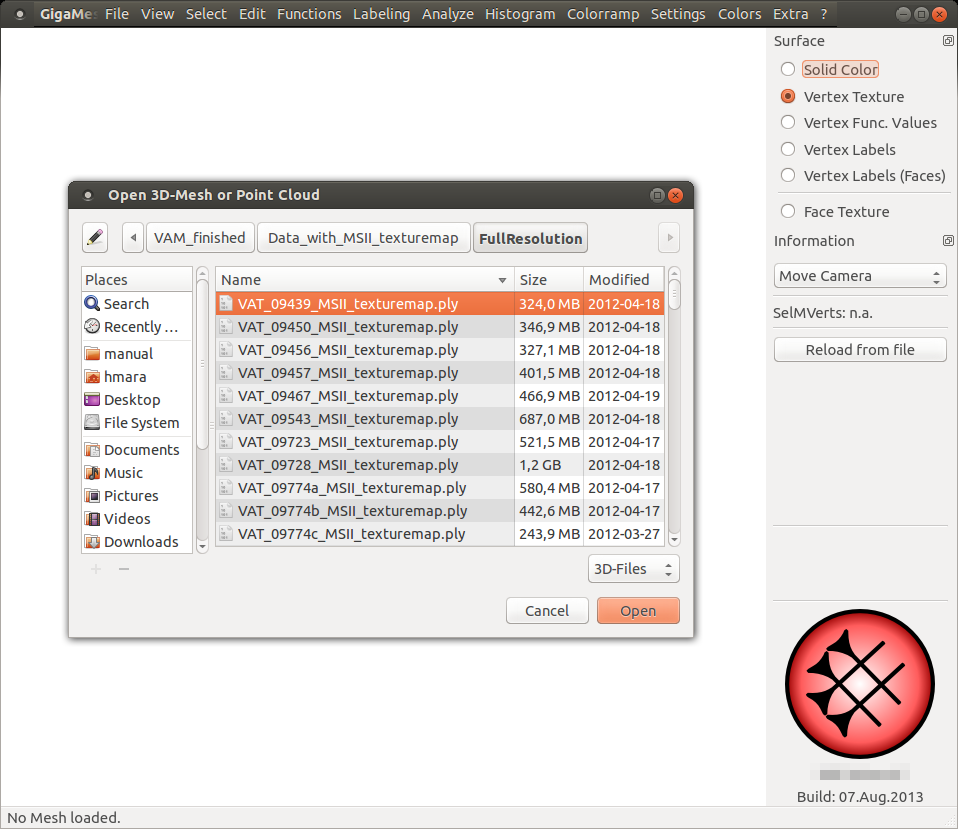
\includegraphics[width=10cm]{figs/gigamesh_gui_startup}
    \caption{Start up of \GigaMesh}\label{fig_start}
\end{center}
\end{figure}

\paragraph*{Step 2}
Orient the model with the help of the mouse or the keyboard (\keystroke{Q}/\keystroke{E} for roll (counterclockwise (CCW) or clockwise (CW) rotation about z-axis) by 1°; \keystroke{W}/\keystroke{S} for yaw (CCW/CW rotation about x-axis) by 1°; \keystroke{A}/\keystroke{D} for pitch (CCW/CW rotation about y-axis) by 1°). This step is needed later on for a proper six side view.

\begin{figure}[H]
 \centering
 \begin{tabular}{cccc}
  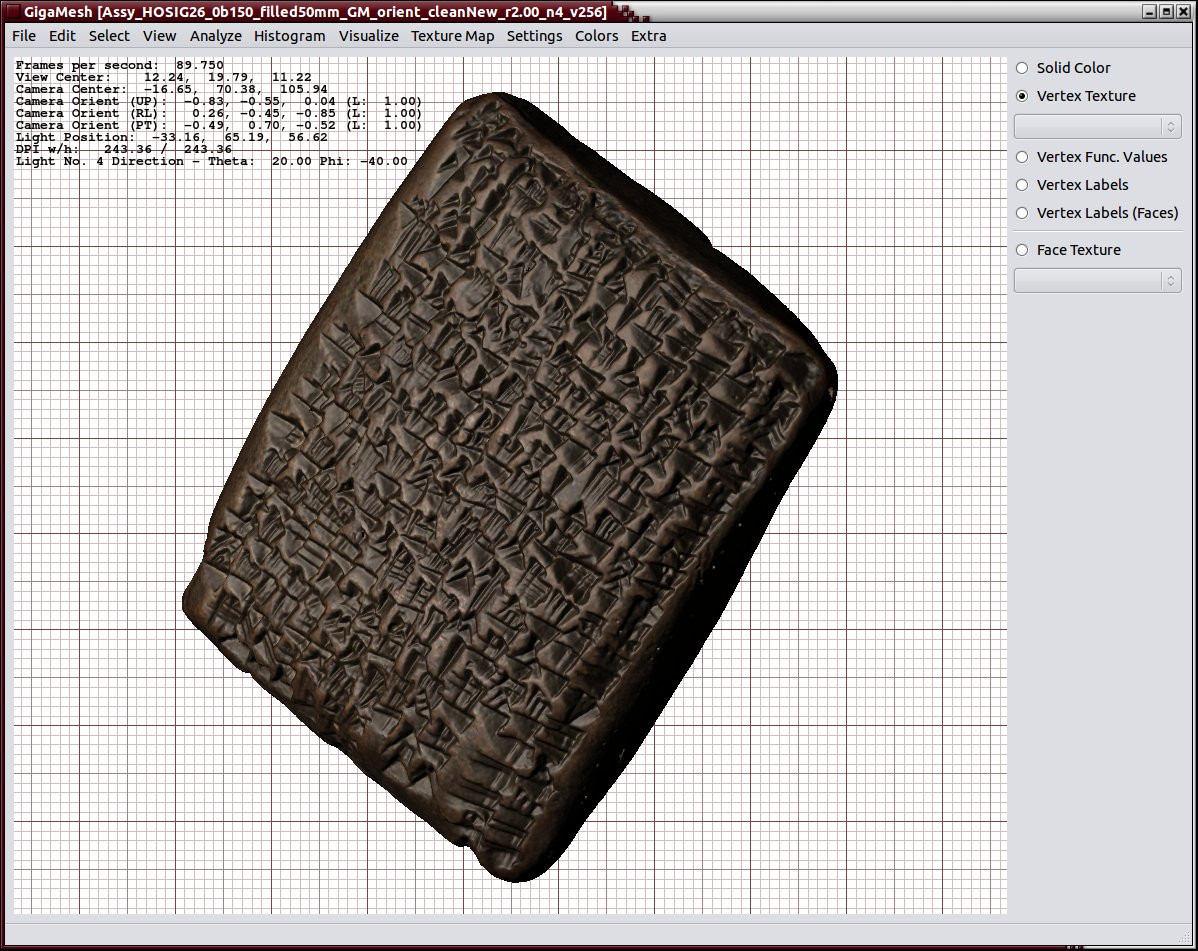
\includegraphics[width=3cm]{figs/not_oriented_01} & 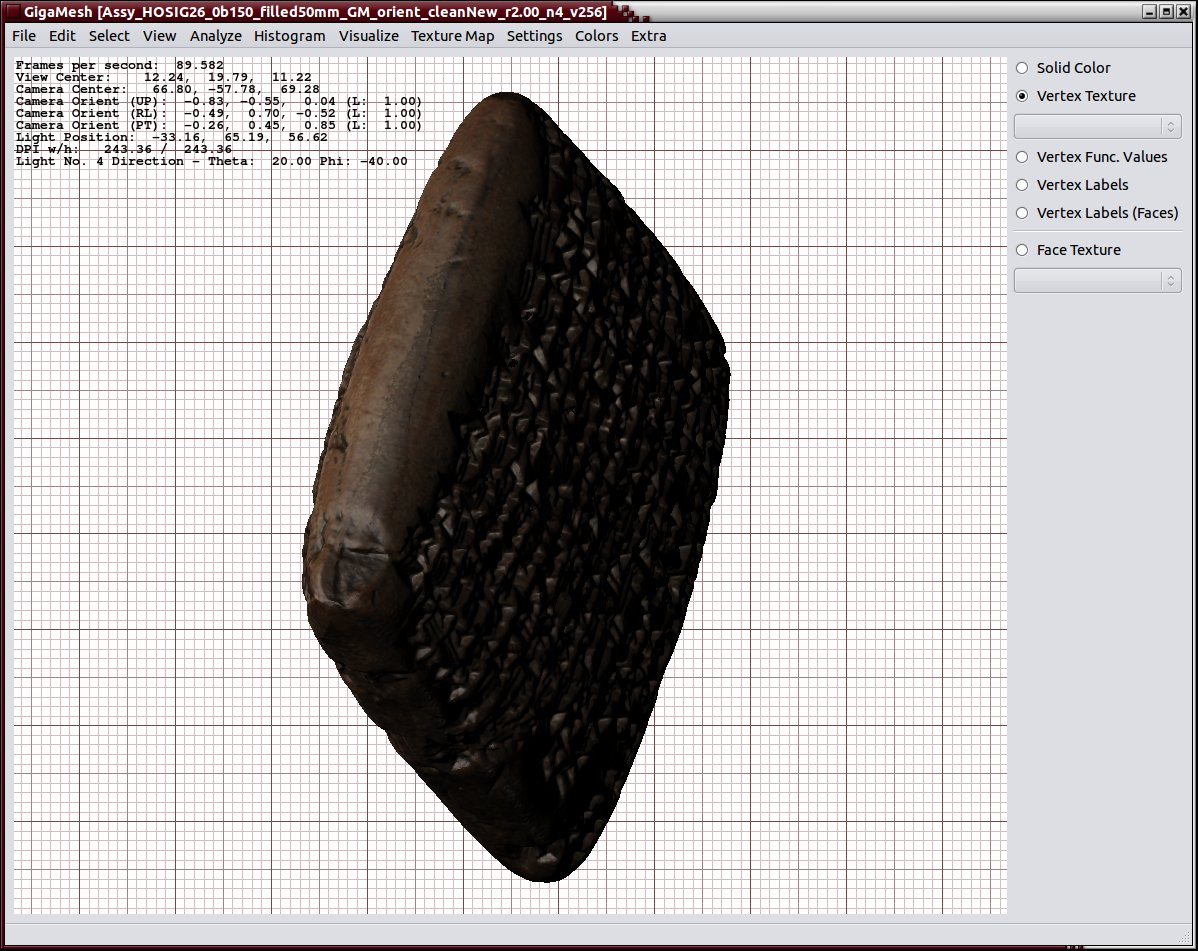
\includegraphics[width=3cm]{figs/not_oriented_02} & 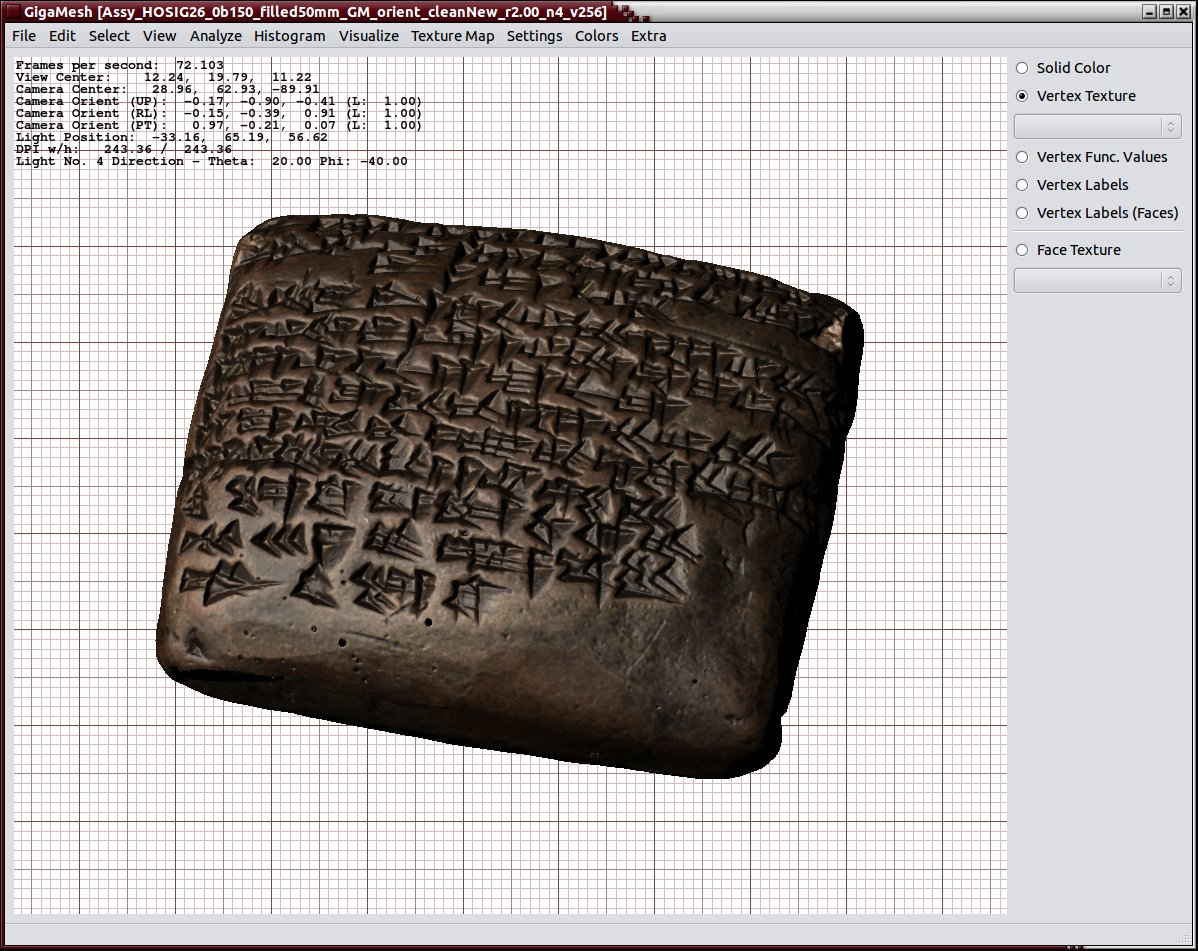
\includegraphics[width=3cm]{figs/not_oriented_03} & 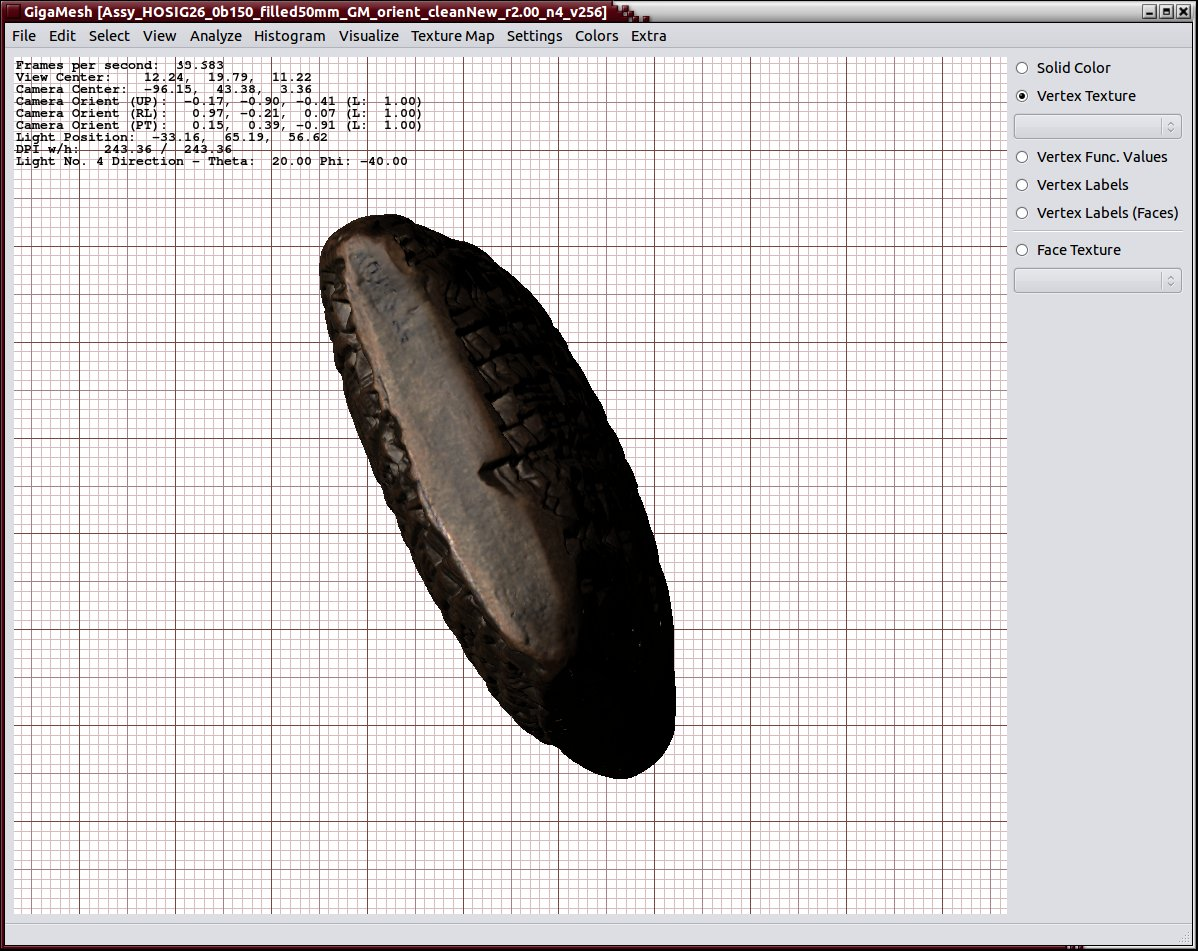
\includegraphics[width=3cm]{figs/not_oriented_04} \\
  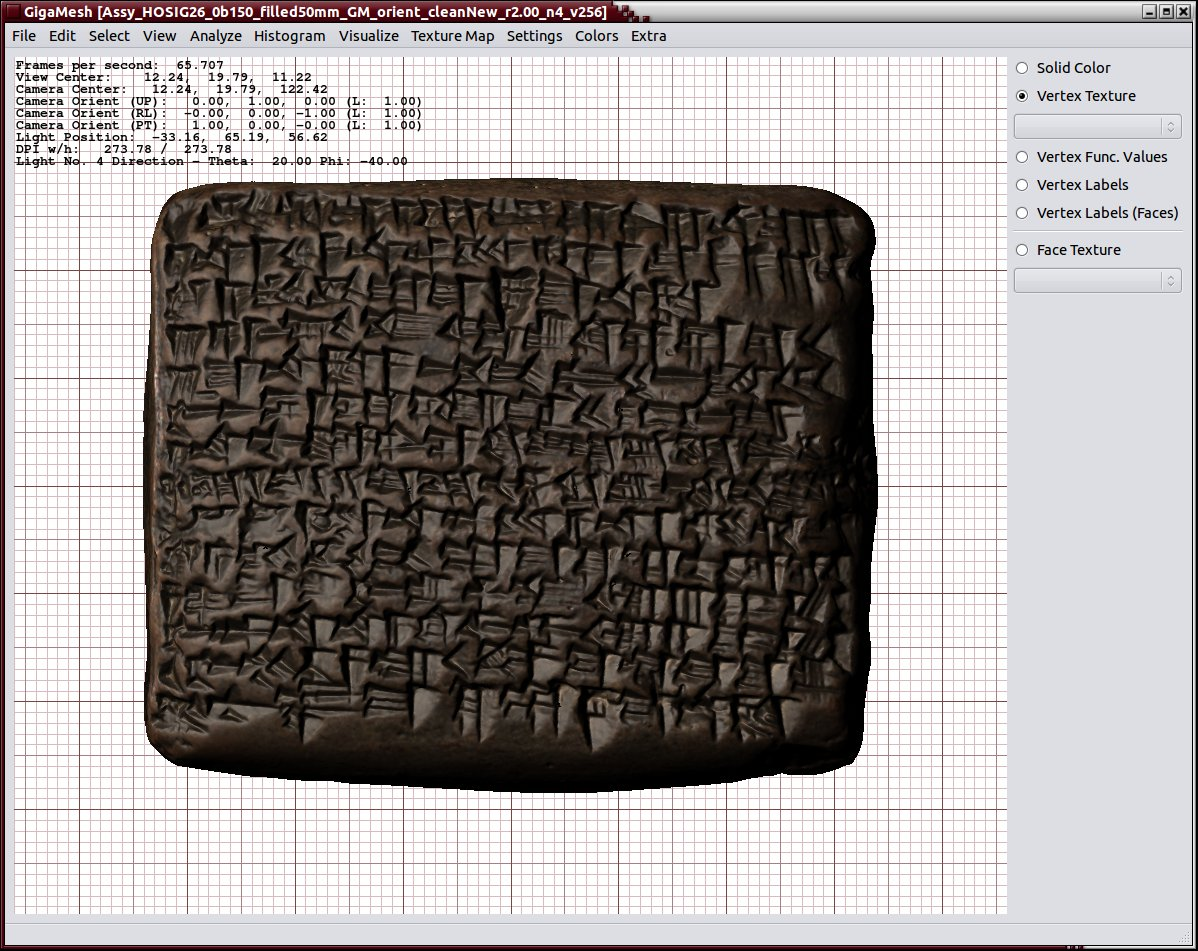
\includegraphics[width=3cm]{figs/oriented_01} & 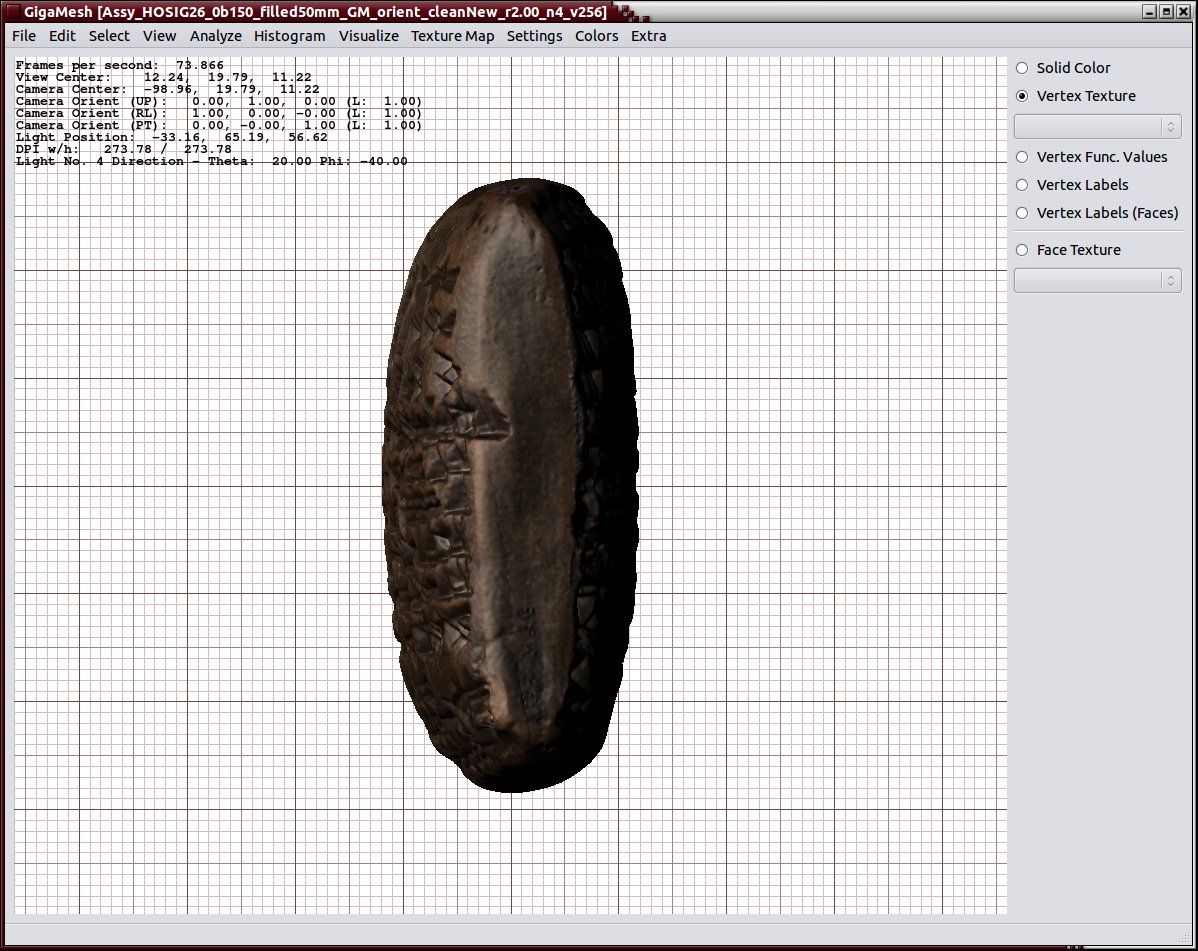
\includegraphics[width=3cm]{figs/oriented_02} & 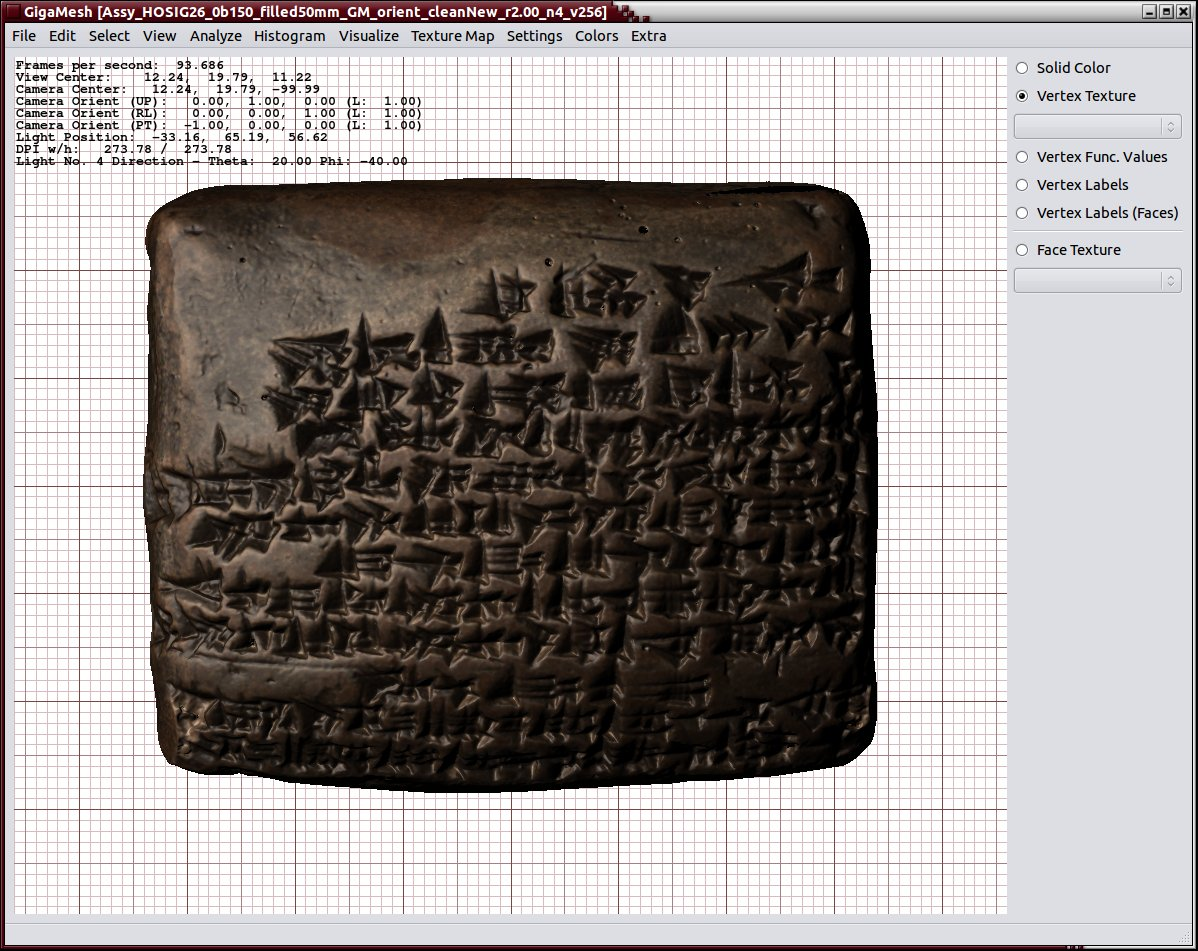
\includegraphics[width=3cm]{figs/oriented_03} & 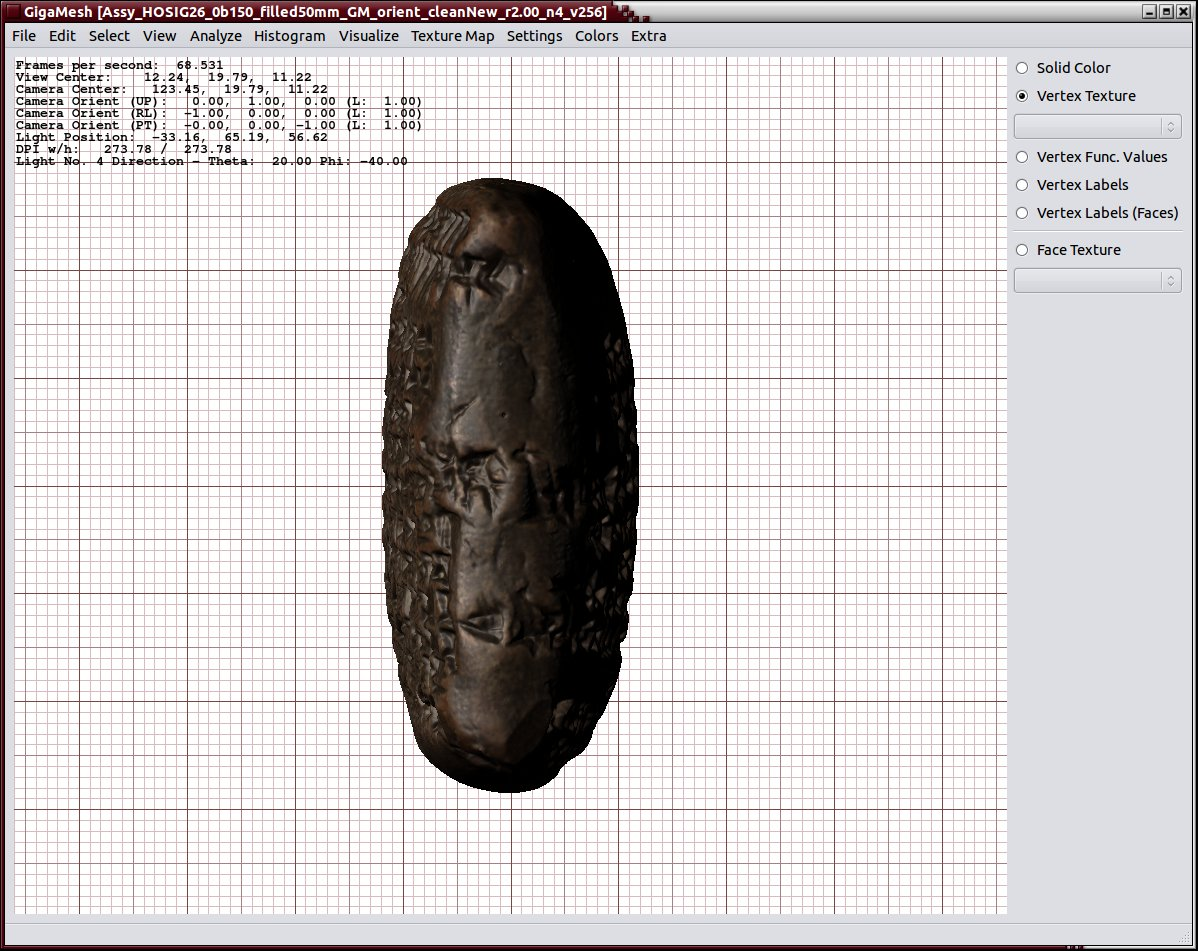
\includegraphics[width=3cm]{figs/oriented_04}
 \end{tabular}
  \caption{not oriented (upper row) and oriented (lower row) version}
\end{figure}

With the help of \keystroke{Y}/\keystroke{X} (pitch by 90 °), \keystroke{C}/\keystroke{V} (yaw by 90 °) and \keystroke{B}/\keystroke{N} (roll by 90 °) it is possible to check if all sides of the object are oriented correctly.
When finished and happy with the result, press \!\keystroke{F6} to save the current orientation matrix. If you do additional  transformation you are now able  to recover this saved orientation by pressing \!\keystroke{F12} or \!\keystroke{Shift} + \!\keystroke{F12}\!, respectively. Now save the whole file with \texttt{File} $\rightarrow$ \texttt{Save As}. As a naming convention extend the filename by {\tt \_GMO} for \GigaMesh Oriented.

\paragraph*{Step 3}
Next the feature vectors have to be calculated. These vectors contain additional information per vertex concerning surface and volume of a set of spheres intersecting the mesh. See \cite{Mara10c} for more background information on the {\em Multi Scale Integral Invariant }(MSII) filtering technique. This operation is rather time consuming (it takes hours or even days of computing time) and therefore better runs without graphical user interface. Open a terminal and change into the \texttt{GigaMesh/mesh/} folder (with the help of the \texttt{cd} command). There should be an executable called:
\begin{center} \texttt{featurevectorthreads\_25d} \end{center}
%without any ending or with .o as an ending (or rather: does the folder contain an executable with this name?). If so, skip Step 4 and proceed with Step 5.
%\paragraph*{Step 4}
If the folder contains no executables then they still have to be compiled (see \ref{FAQ}).

\paragraph*{Step 4}
Type 
\begin{center} \texttt{./meshgeneratorfeaturevectors25d\_threads -f <path-to-filename> [-r 2]} \end{center}
For \texttt{path-to-filename} the (relative or absolute) path to the folder of the data file and the name of the data file to be visualized has to be given. The parameter given behind the option {\tt -r}  displays the radius of the maximal sphere for the MSII filter. The default value has been set to the unit $1.0$.  It  can be changed into some other appropriate number depending on the size of the features to be detected. An educated guess is the maximum size of the feature width. Smaller values will only detect noise and bigger values lose the fine tuning when operating with the feature vectors in \GigaMesh\!\!.
Note again that depending on the filesize of the object this step can take several hours. Finally there should have appeared a data file named  
\begin{center}
{\tt filename\_r2.00\_n4\_v256.ply} 
\end{center}
due to naming conventions which contains the feature vectors and can be processed by \GigaMesh in the next steps. For more information see chapter \ref{tasks}.

\paragraph*{Step 5}
To proceed with the visualization switch to \GigaMesh\!\!'s GUI and load 
\begin{center} \texttt{filename\_r2.00\_n4\_v256.ply} \end{center}
This is the object already containing the feature vector. 
Now select the deepest wedge on the surface of the object by double clicking it with the left mouse button. Next go to \texttt{Functions $\rightarrow$ Feature Correlation to SelVert}.
\begin{figure}[H]
\begin{center}
    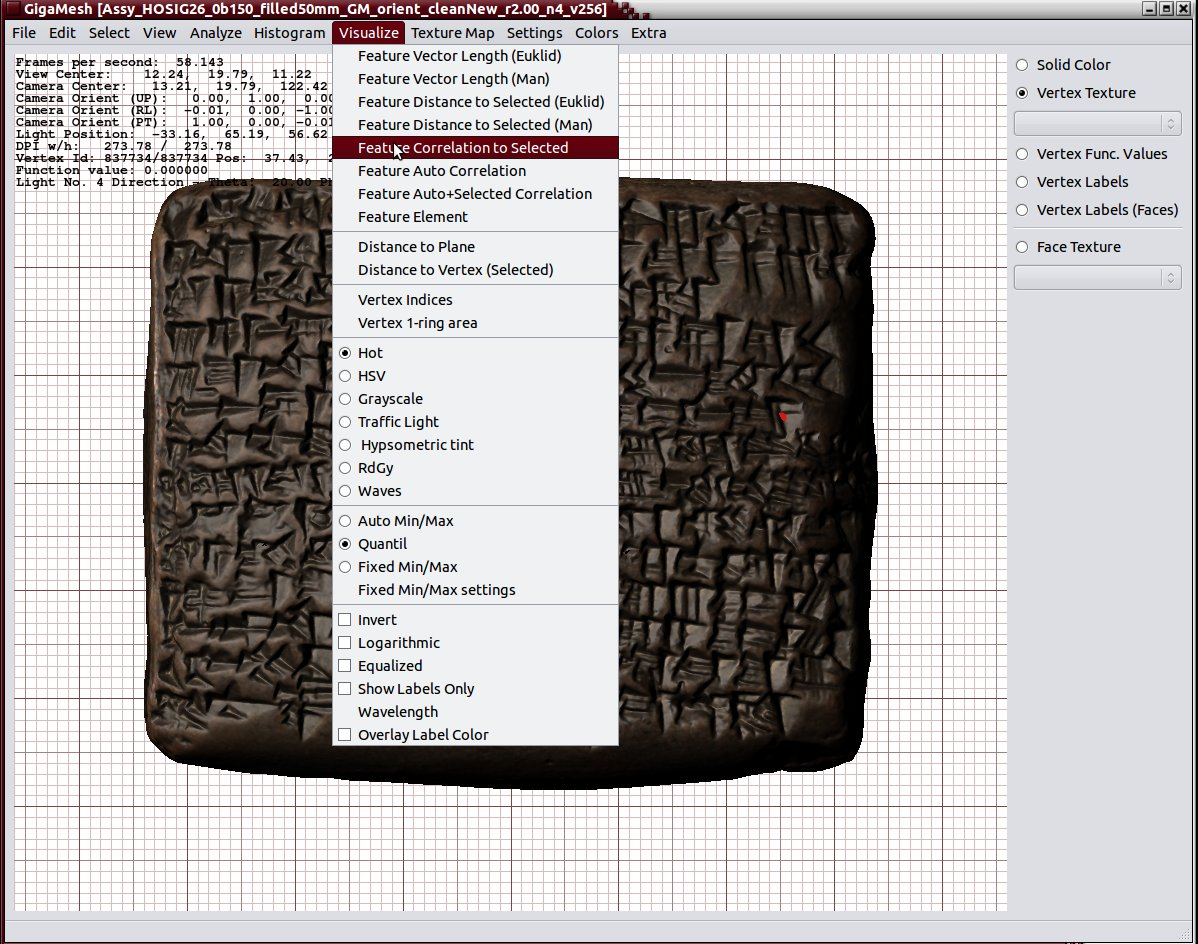
\includegraphics[width=10cm]{figs/Feature_Correlation}
    \caption{Selected Vertex (red dot) and dropdown menu for feature detection}
\end{center}
\end{figure}
Please note that this step may take several minutes before it is completed. The default colormap is the so-called {\tt Hot}, displaying the a ramp from dark red to orange to light yellow.

\paragraph*{Step 6}
Colors can be modified to \texttt{Colorramp $\rightarrow$ Grayscale}. Next click \texttt{Colorramp $\rightarrow$ Invert} which inverts all the colors or shades of gray. Switch off the light with \keystroke{0}\!. If necessary double click somewhere empty for deselection and refresh. What you see is the coloring of the surface according to the curvature and without any lighting active. Of course you may switch on the light again with \keystroke{0} and also manipulate the lights  with  \keystroke{1} to  \keystroke{5} and pressing the ctrl-key while moving the mouse. This enhances the realistic impression.
%Now the visualization of the object with the feature vector is finished.
\begin{figure}[H]
 \centering
 \begin{tabular}{cccc}
  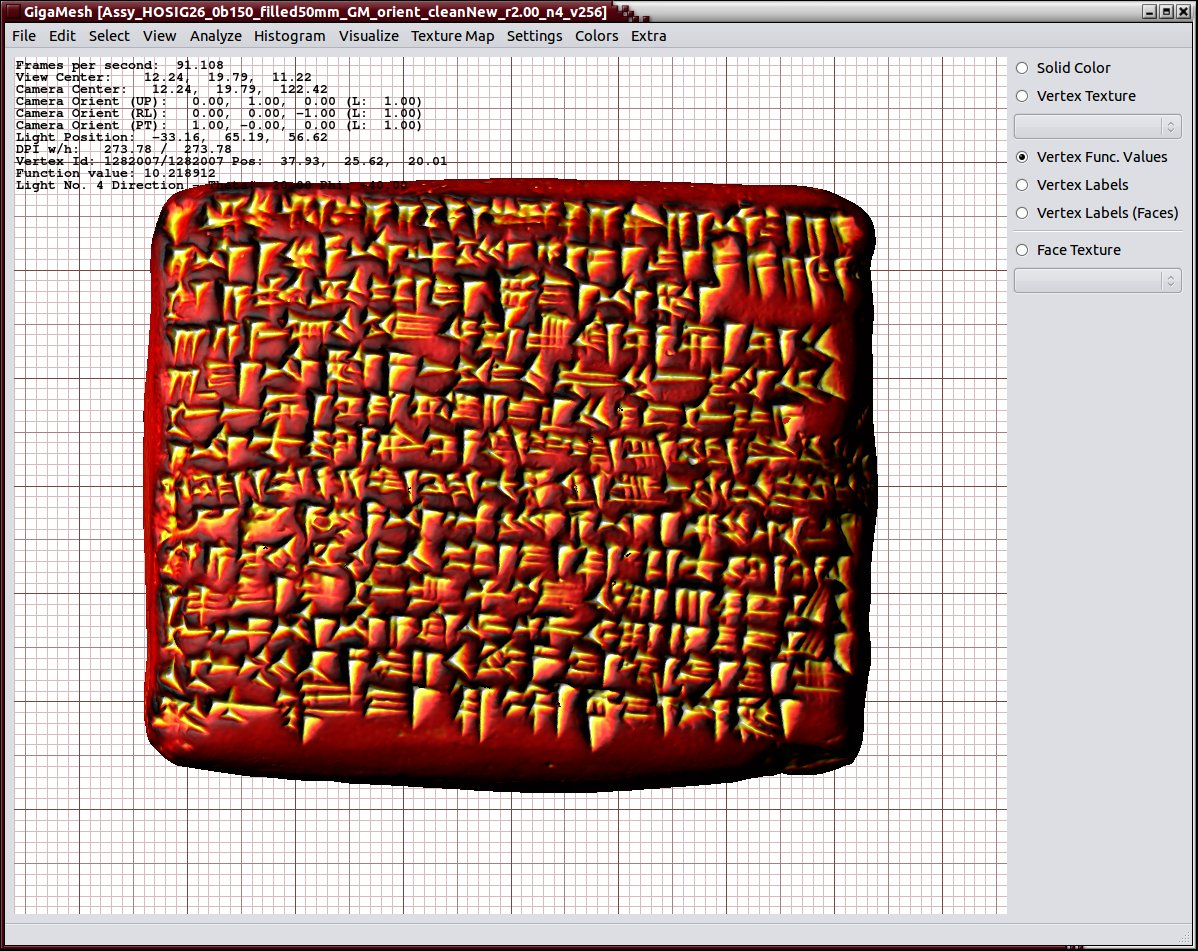
\includegraphics[width=3cm]{figs/featvecthotcorr} & 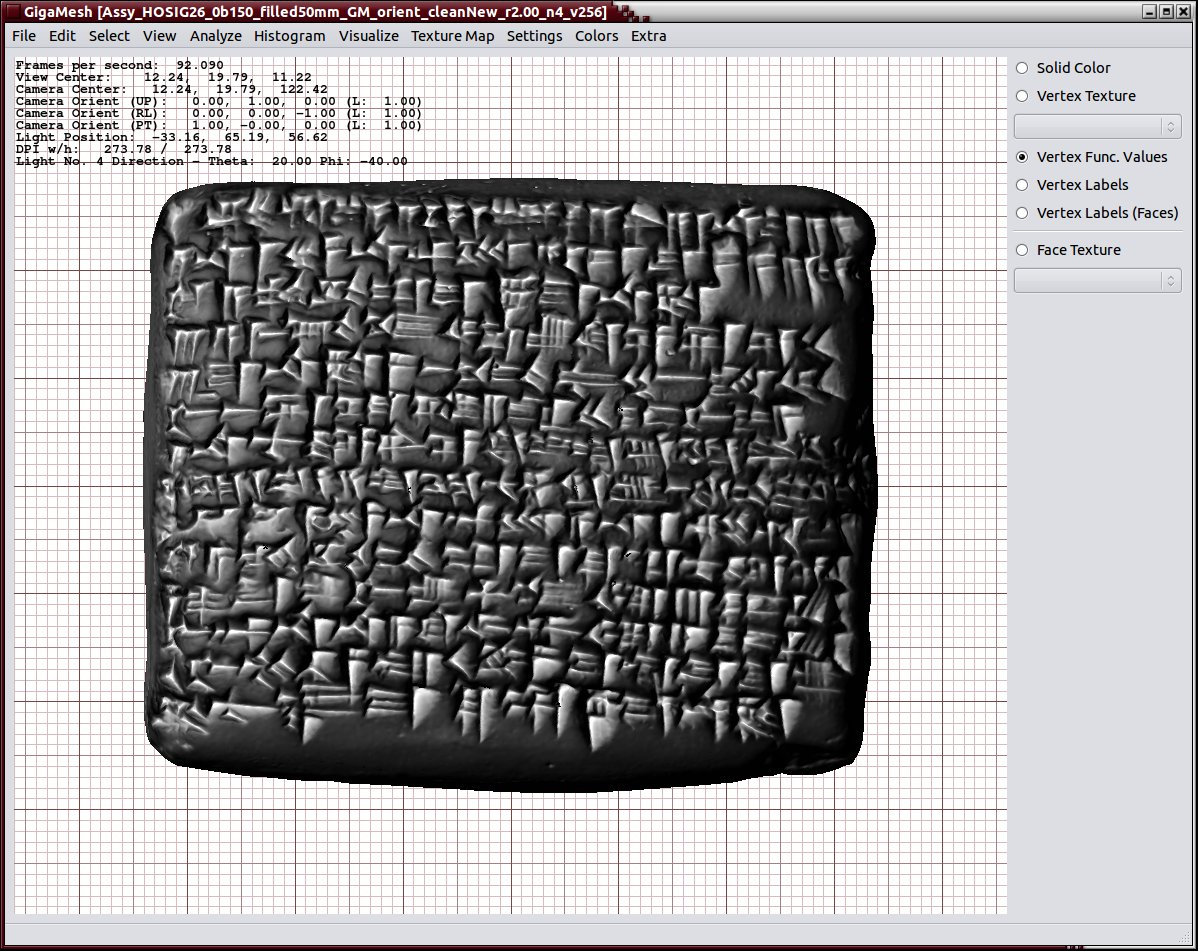
\includegraphics[width=3cm]{figs/featvectgrayscale} & 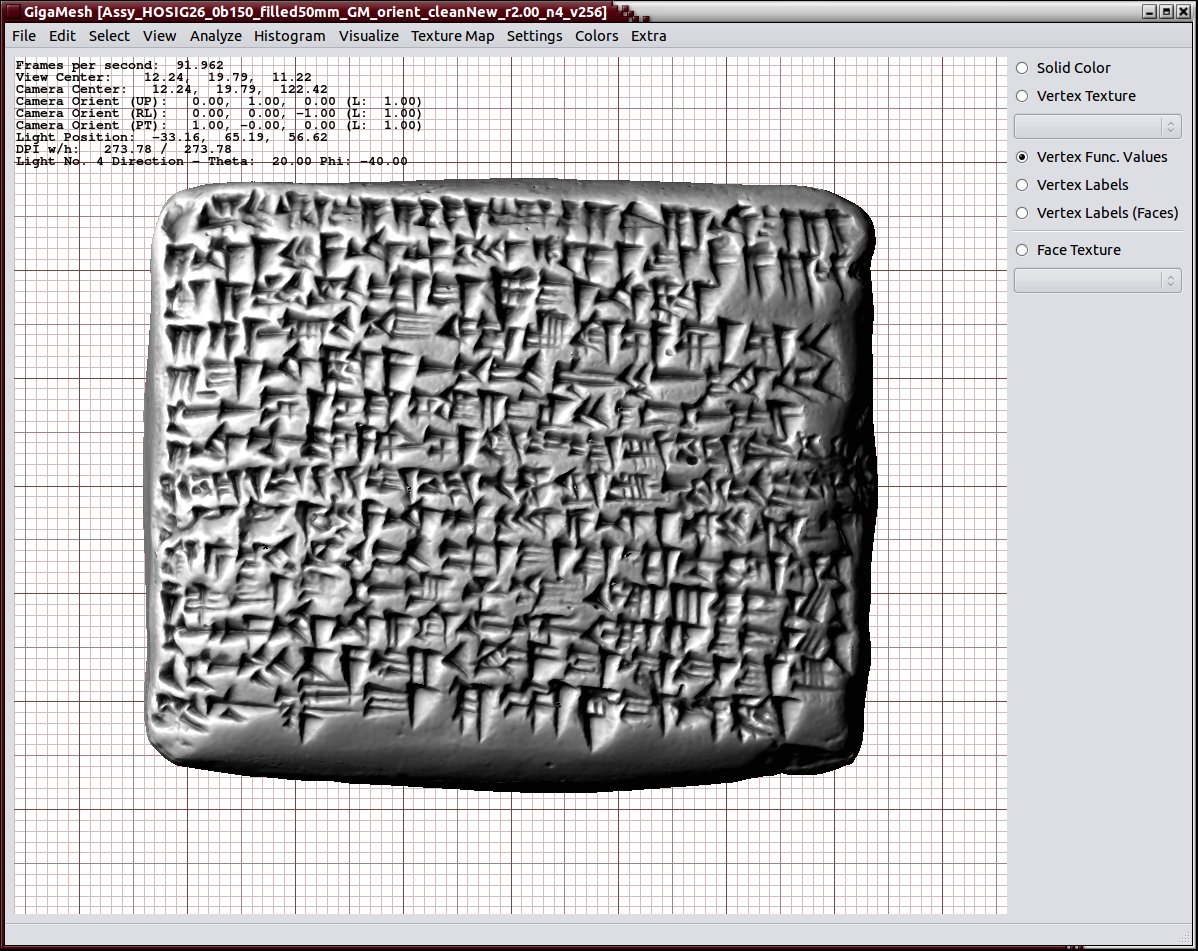
\includegraphics[width=3cm]{figs/featvectgrayscaleinverted}
  & 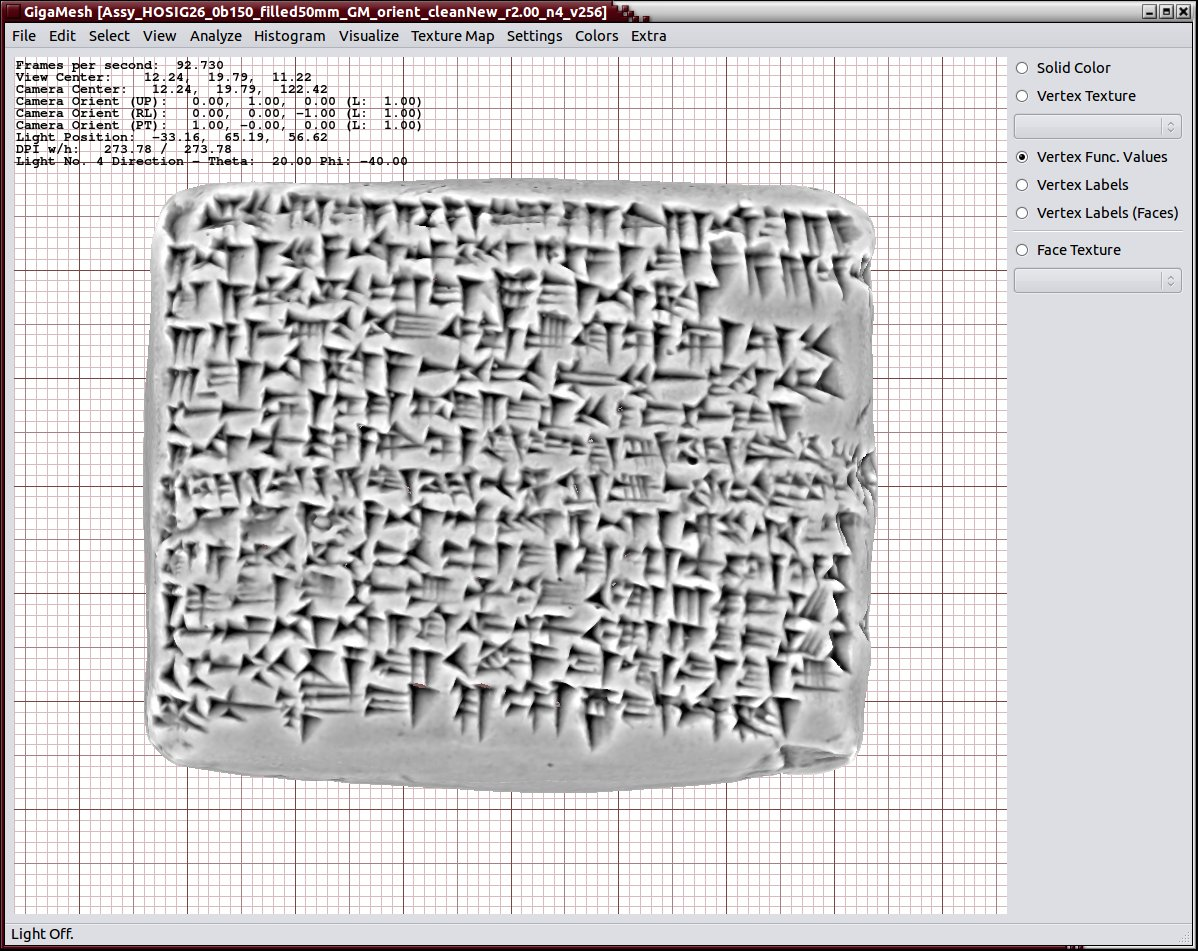
\includegraphics[width=3cm]{figs/featvectgrayscaleinvertedwolight}
 \end{tabular}
  \caption{From left to right: Object with feature vector in hot correlation display, then in grayscale, in inverted grayscale and in inverted grayscale without light}
\end{figure}

%\pagebreak
\paragraph*{Step 7}
To do a six side view of the above visualized object go to \texttt{Settings $\rightarrow$ Ortho Scale (Set DPI)} and set the resolution. A good help for the right resolution is to check the terminal (see marked part in picture 3.5 below) and set the value a little bit above the one in the terminal. E.g.~in this example the terminal says 545.068 DPI, so it is good to set it to about 600 DPI.
\begin{figure}[H]
\begin{center}
    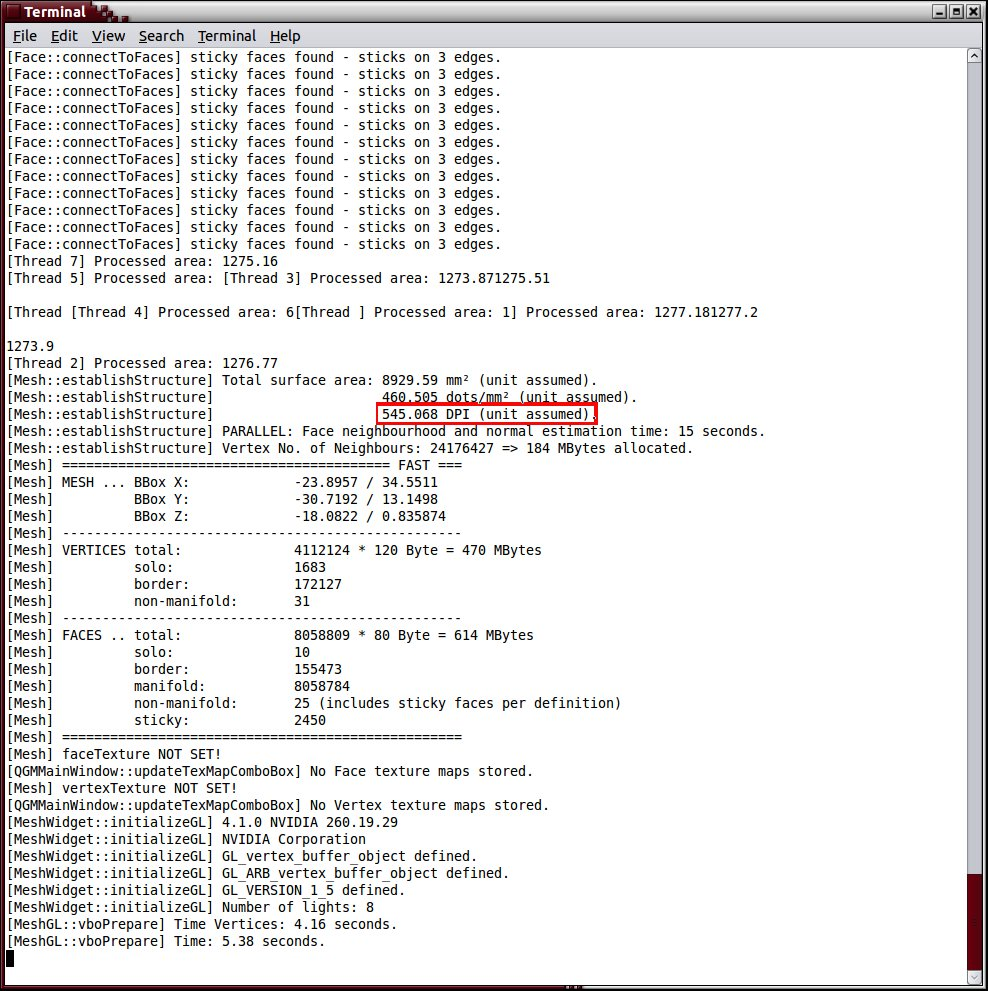
\includegraphics[width=10cm]{figs/Terminal02}
    \caption{The DPI of the file marked with red.}
\end{center}
\end{figure}

%\pagebreak
Then hit \texttt{File $\rightarrow$ Export Screenshots $\rightarrow$ Screenshot Views} and answer the question for tiled rendering with yes. 
For the optional export of the information into a \LaTeX file go to \texttt{Extra $\rightarrow$ Cuneiform Figure Latex Info}.
\tabletfatcross{HOSIG 26 -- 6 views, scale $1:1.5$}{figs/HOSIG26_GMOCF_perfect_r201_n4_v256}{0.667}{fig:HOSIG26}
%\tabletfatcross{HOSIG 26 -- 6 views, scale $1:1.5$}{figs/Assy_HOSIG26}{0.667}{fig:HOSIG26}
\begin{center}
	\begin{tabular}{cc}
		\begin{tabular}{|l|r|}
			\hline
			Max. dim.       & $\numprint{6.8} \times \numprint{5.7} \times \numprint{2.4} \,cm$ \\
			\hline
			Vertices        & $\numprint{1628456}$ \\
			Faces           & $\numprint{3255868}$ \\
			\hline
			Material        & \multicolumn{1}{l|}{} \\
			\hline
		\end{tabular}
		\begin{tabular}{|l|r|}
			\hline
			Surface, acq.    & $\numprint{10765}\,mm^2$ \\
			\hline
			Res., avg       & $\numprint{151}\,mm^{-2}$ \\
			                & $\numprint{312}\,DPI$ \\
			\hline
			Volume, est.    & $\numprint{61}\,\pm\numprint{1}\,cm^3$ \\
			\hline
		\end{tabular}
	\end{tabular}
\end{center}



\section{Ceramics}\label{vessels}

\GigaMesh features the possibility to create cutting planes. In order to get the proper outline of, e.g.~a vessel, this possibility sets a plane inside the vessel and ``cuts'' the object thereby showing its outline.

The first step is to \texttt{Select $\rightarrow$ Plane - 3 Points)} where the user will define a plane by three points: mark three points on the plane with three doubleclicks. The plane can be shown with \texttt{View $\rightarrow$ Mesh Plane}. In theory this plane is movable. Then calculate the distance to the plane. By selecting \texttt{Analyze $\rightarrow$ Iso Lines to Polylines} the value for Isovalue should be set to 0. Then with \texttt{File  $\rightarrow$ Export Screenshots $\rightarrow$ Screenshot (SVG + PNG)} of the current view. This projects the polygonal lines  to screenshots and calculates the outline.
\begin{figure}[H]
\begin{center}
    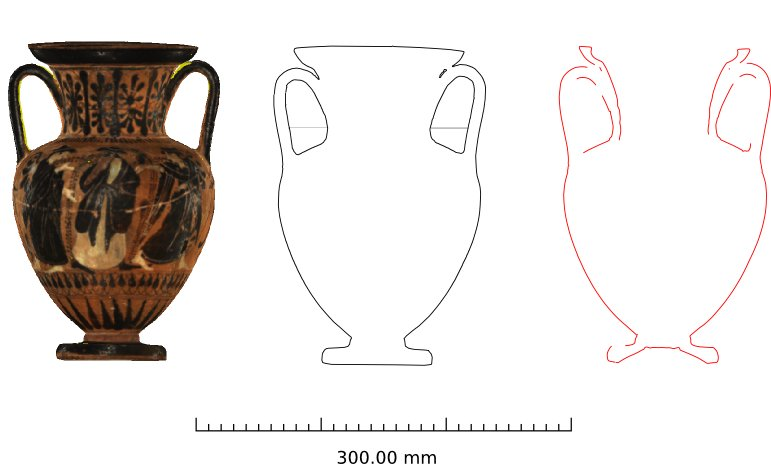
\includegraphics[width=12cm]{figs/IV_670_1}
    \caption{Vessel and its cutting planes}
\end{center}
\end{figure}